\subsection{Plots}

% include: 
% filtered data
% thresholds
% R peaks
% regions with unstable rythm
% searchback

The resulting data from the program is shown in figure \ref{fig:10k_points}.\footnote{To see how the filters alter the original data, step-by-step see Appendix \eqref{Apx:A}}

\begin{figure}[H]
    \centering
    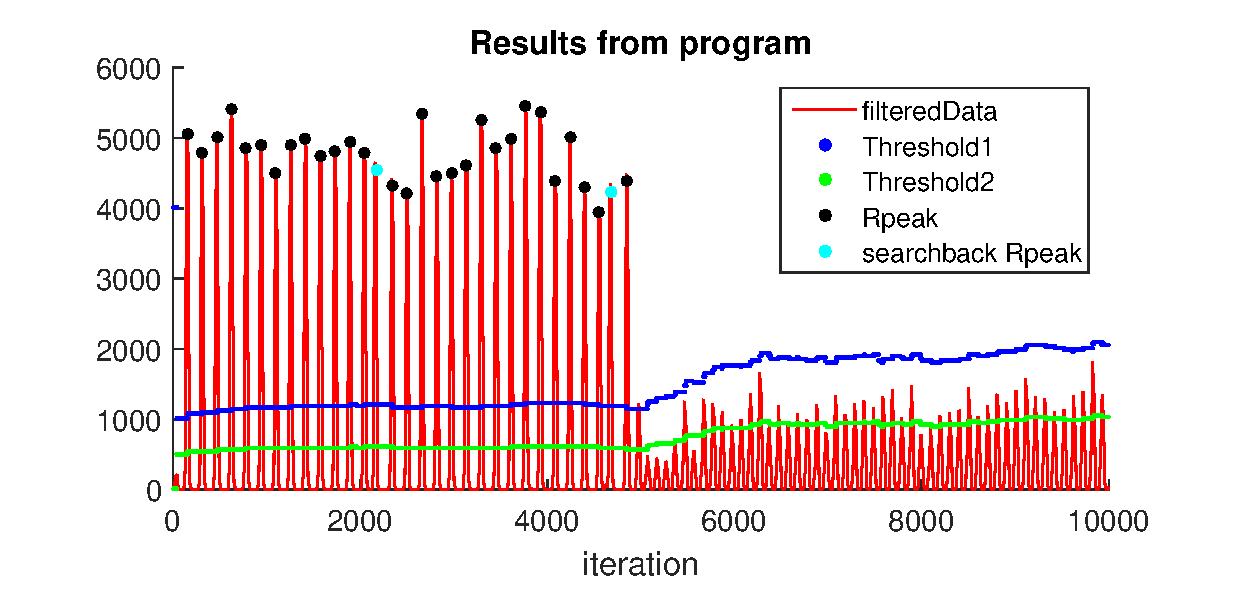
\includegraphics[width=1.0\textwidth]{3Results/fig/10kpointsmatlab.eps}
    \caption{Results from the program, plotted in \texttt{MATLAB}. The thresholds automatically adjust to ignore the noise peaks following the heart failure at iteration $\approx$ 5000. 31 peaks are found (blue, black), 2 of them through searchback (black). }
    \label{fig:10k_points}
\end{figure}

For the first 5000 data points we see that we find Rpeaks and our thresholds are acceptable. Two peaks are found during searchback, at around iteration 2100 and 4500. This would suggest that the peaks come either faster or slower than expected; missing the \texttt{RR\_LOW} to \texttt{RR\_HIGH} interval. After 5000 data points the heartbeat gets alarmingly weak and the thresholds are adjusted. This adjustment is caused by the program recognizing the signal as noise and not accepting the input as Rpeaks.\\
\\
If we look closer in at around iteration 5000 we get figure \ref{fig:1kpoints}.

\begin{figure}[H]
    \centering
    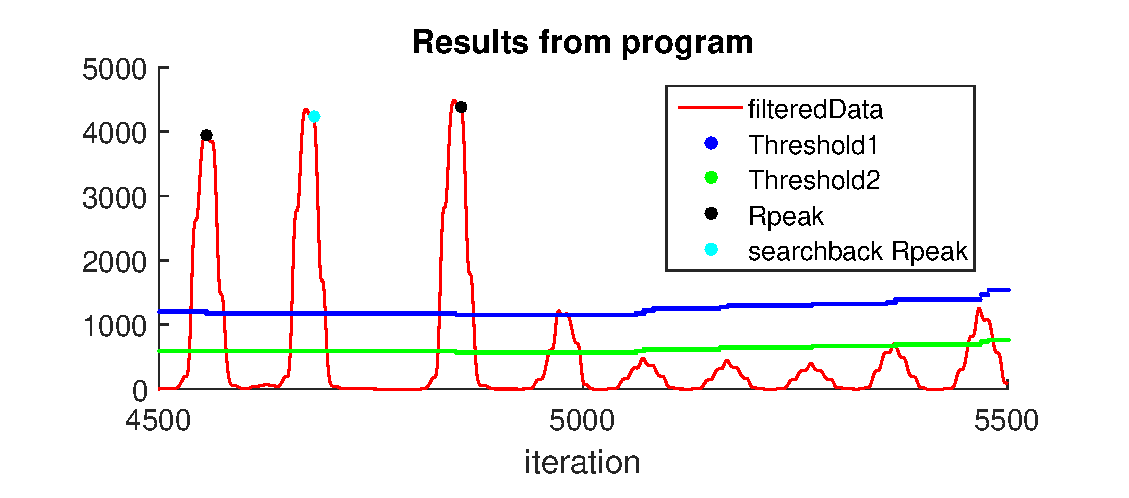
\includegraphics[width=1.0\textwidth]{3Results/fig/1kpointsmatlab.eps}
    \caption{Results from the program, where the peaks found correspond to (local) maxima in the filtered data. If a peak in the filtered data has two smaller peaks, the searchback function finds the latest, i.e. the subpeak at the highest iteration.}
    \label{fig:1kpoints}
\end{figure}

In figure \ref{fig:1kpoints} we see the position of the Rpeak, and how under normal conditions the program detects the first peak (main peak) but in searchback it detects the second peak (subpeak). When the algorithm begins searchback, a new peak stronger than \texttt{THRESHOLD1} must be found first (see figure \ref{fig:QRS_flowchart}). After searchback is executed, the peak (at which the program began searchback from) is ignored, and the next peak found is the subpeak. This results in the subpeak being stored as Rpeak after every searchback, as seen on figure \ref{fig:10k_points}.\\ Figure \ref{fig:1kpoints} shows how the filters has minimized noise between peaks.\\
\\
In figure \ref{fig:comparing_peaks}, we compare our data with the expected output\footnote{The expected output is generated by Nicolai Pedersen, project supervisor.}. we see a clear resemblance, with an average error of 0.4 $\%$, and a maximum error of 4.5 $\%$. Implementations of the filters are known to be different from the expected program structure to our program structure. Our implementation postpones integer division to minimize division error. The differences in results are also at different iterations suggesting that the error is caused by finding different peaks (main peak vs. subpeak).

\begin{figure}[H]
    \centering
    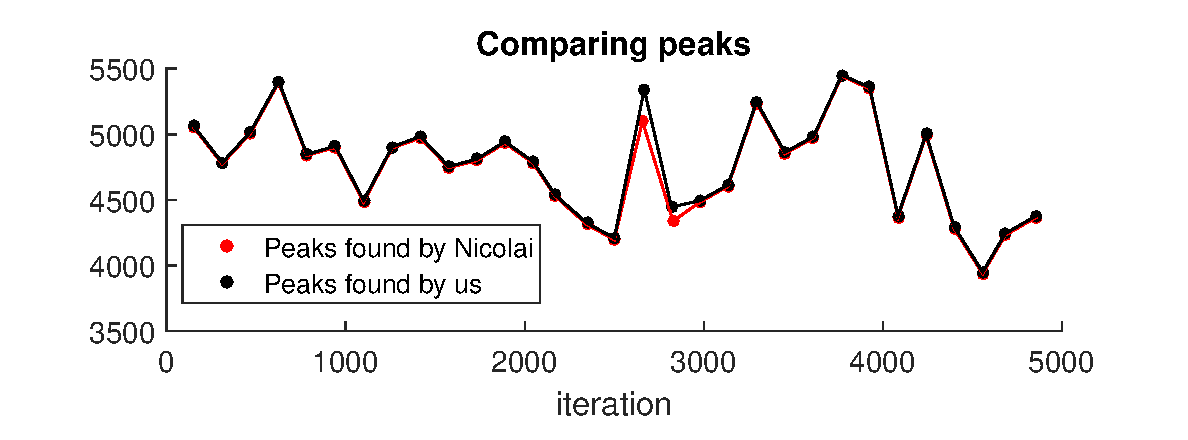
\includegraphics[width=1.0\textwidth]{3Results/fig/comparingPeaks.eps}
    \caption{When comparing our 31 peaks found to those found by Nicolai Pedersen, there is an overall resemblance. The mean absolute difference between red and blue peaks is 0.4 $\%$. The largest different (4.5 $\%$) occurs at iteration 2667. We connected the points to make the graph faster to read.}
    \label{fig:comparing_peaks}
\end{figure}
